
This study is designed as a detailed comparison of CNN-based models, with and without \diff\ in input, with the results from one RB model, \texttt{autoscan} \citep{Goldstein_2015}. The choice of \texttt{autoscan} as our point of reference is motivated by its application to the discovery of transients in a state of the art facility, the Dark Energy Survey \citep{DES}, which can be considered a precursor of upcoming surveys like the Rubin Legacy Survey of Space and Time \citep{ivezic2019lsst}. The latter,  expected to start in 2024, will deliver $\sim 20~\mathrm{Tb}$ of high resolution sky image data each night, covering a footprint of $\sim20,000$ sq. deg. every $\sim 3$ nights, with expected millions of transients per night, demanding rapid methodological and technical advances in accuracy and efficacy of transient detection models.


%\section{
% The data used in this project consists of images collected by The Dark Energy Survey during its first observational season, August 2013 through February 2014. The data corresponds to observations of $898,963$ transients labeled by human inspection in two groups (\textit{OBJECT\_TYPE}): $454,092$ are labeled as real astrophysical transients ($1$) and $444,871$ as artifacts, or ``bogus'', as it is customary in the field,. Three images are made available for each transient, each of size $51 \times 51$, divided in three groups: the template (\temp) images, science images (\search) and the difference (\diff) images, correspond to the result of subtraction of template and science images [\cite{Goldstein_2015}]. Every group of three images (\diff,\search,\temp) correspond to a unique 'ID' and each one of the images has the same label information encoded in a binary 1 or 0 for ``real'' and ``bogus'' respectively.
% %}
% All the information about this training instances can be found in \url{https://portal.nersc.gov/project/dessn/autoscan/#}.\\




The data used in this work consists of postage stamps of images collected by the DES during its first observational season (Y1), August 2013 through February 2014\footnote{The data can be found in \url{https://portal.nersc.gov/project/dessn/autoscan/\#}} \citep{Abbott_2018}. The data corresponds to 898,963 DIA-sets, a template (\temp) image, search (\search) image, and their difference (\diff). The construction of the templates images for the DES Y1 leveraged the data collected in season two (Y2) as well as the Science Verification images (observations collected prior to survey start in order to evaluate the performance of the instrument). More information on the DES DIA pipeline can be found in \citep{Kessler_2015}.  Of these DIA sets, 454,092 contain simulated SNe Ia, which constitute the ``real'' astrophysical transients set (\texttt{label = 0}) and 444,871 are the actual data from DES, \ie, the ``bogus'' set (\texttt{label = 1}). Each image is offered in two formats: ``.gif'', and ``.fits''. The former is an 8-bit compressed format (convenient for visual inspection as it can be opened with commonly available software); the latter, the ``Flexible Image Transport System'', is a common data format for astronomical data sets which enables high precision with a large dynamic rage. The data in ``.fits'' format was used in this work.\footnote{More information related to how to manipulate this astronomical data format is available in \url{https://docs.astropy.org/en/stable/io/fits/}} Each image is $51 \times 51$ pixels - corresponding to approx 0.26 
arcseconds square of sky. 

 Some examples of the data are in \autoref{fig:examples_no_normalization}. Each transient is identified by a unique ``ID''. The metadata, includes the labels associated with each image as well as the the $38$ features used for classification in \citet{Goldstein_2015}.
 Because we only analyze postage stamps with detections, we implicitly still rely on the DIA to enable the detection step at this stage of our work. The \temp\ and \diff\ image in our postage stamps, however, are not PSF matched.
% \\
% \vspace{-10.8mm}


 %The other two columns corresponded to the ``ID'' and the ``OBJECT$\_$TYPE'': ``real'' (0) and ``bogus''(1); these two were used for this work.
\subsection{Scaling and normalization}\label{subsec:scaling}


A word about data preparation and normalization is in order as  astrophysical images are inherently very different from the images upon which CNNs have been built. When training CNN models for image analysis, each image is typically simply scaled to a common range ($0-1$). However, the dynamic range of an astrophysical image is typically large and the distribution of pixel values is generally very different from Gaussian, with the majority of pixels sitting at low values (the sky) and a few pixels at or near saturation (which in some cases may carry the majority of the information content). 
Furthermore, in the DIA-set case, the pixel-value distribution of the \diff\ differs qualitatively from the \temp\ and \search\ ones. While the \temp\ and \search\ are typically naturally positive valued with a long tail at the bright end (right-skewed because of the presence of bright astrophysical sources such as galaxies that host transients or stars that vary), the \diff\ image is, in absence of variable or transient sources, symmetric around 0.

%To gave more relevance to the 
The \diff\ images %and for their Gaussian behavior, as seen in \autoref{fig:histobeforenormalizarion} (first left column); each of them was
were standardized % The \diff\ images would 
to have a mean $\mu = 0$ and a standard deviation $\sigma = 1$. The \search\ and \temp\ images, instead, were scaled %minimum and maximum value for each image and considering pixel values inside the 
to map the $\mu\pm 3\sigma$ interval of the original image to $0-1$. %Meaning that $mean \pm 3\sigma$ would be $0$ or $1$ respectively. However, 
This scheme allows us to retain resolution in the shape of the core of the distribution while also retaining extreme pixel values. % allows  negative values and values above $1$ because extreme (outside the $3\sigma$ clip) values were scaled too. 
    \autoref{fig:histobeforenormalizarion} shows the distribution of pixel values for four DIA sets, for the same data as in \autoref{fig:examples_no_normalization}, which include two ``real'' and two ``bogus'' labels. \hyperref[sec:appendixa]{Appendix A} shows the pixel distributions before and after scaling for the same data.


% \begin{figure}[H]
%     \centering
%     \includegraphics[width=0.6\linewidth]{
%     figures/histnorm_new_test.pdf}
%     \caption{}
%     \label{fig:histoafternormalizarion}
% \end{figure}




% For the Neural Network Model, the first step was to horizontally stacked each image of each group (already normalized) per ``ID'', following the order (\diff, \search, \temp), and using \textit{np.concatentate}; the size of the data set is then (Number of transient to be considered, $51$, $153$). Some examples are in \autoref{fig:examples_hstack_normalization}. The second step was to have a balance (data set, in which the total of ``real'' (0) and the total of ``bogus'' (1) transient are equal or very similar.  
% \begin{figure}[H]
%     \centering
%     \includegraphics[width=0.4\linewidth]{
%     figures/3dex_new_test.pdf}
%     \caption{Horizontally stacked normalized data for the examples shown in \autoref{fig:examples_no_normalization}. The stacked follow the order, from left to right: (\diff, \search, \temp). Each composite images is normalized as follows, the \diff\ are standarized (subtracting the mean and dividing by the standard deviation); \search\ and \temp\ are preprocessed using the min-max scheme. This is the format of the data input in the neural network (see section \ref{subsection: model_neural_network}).
%     The divergent color map used is \texttt{PRGn}, given by python.} %This images are the final data used for the Neural Network model.  }
%     \label{fig:examples_hstack_normalization}
% \end{figure}

% The training and testing data set without \diff\ images were constructed based on the previous triplet and simply just cutting the \diff\ image.


% \begin{figure}[H]
%     \centering
%     \includegraphics[width=0.35\linewidth]{
%     figures/2dex_new_test.pdf}
%     \caption{Horizontally stacked normalized data for the examples shown in \autoref{fig:examples_no_normalization}. The stacked follow the order, from left to right: (\search, \temp). Each composite images is normalized as follows, \search\ and \temp\ are preprocessed using the min-max scheme. This is the format of the data input in the neural network (see section \ref{subsection: model_neural_network}). The divergent color map used is \texttt{PRGn}, given by python}
%     %The color map used is ``viridis'', given by python. This images are the final data used for the Neural Network model.  }
%     \label{fig:examples_hstack_2Dnormalization}
% \end{figure}


\begin{figure*}

   \centering
   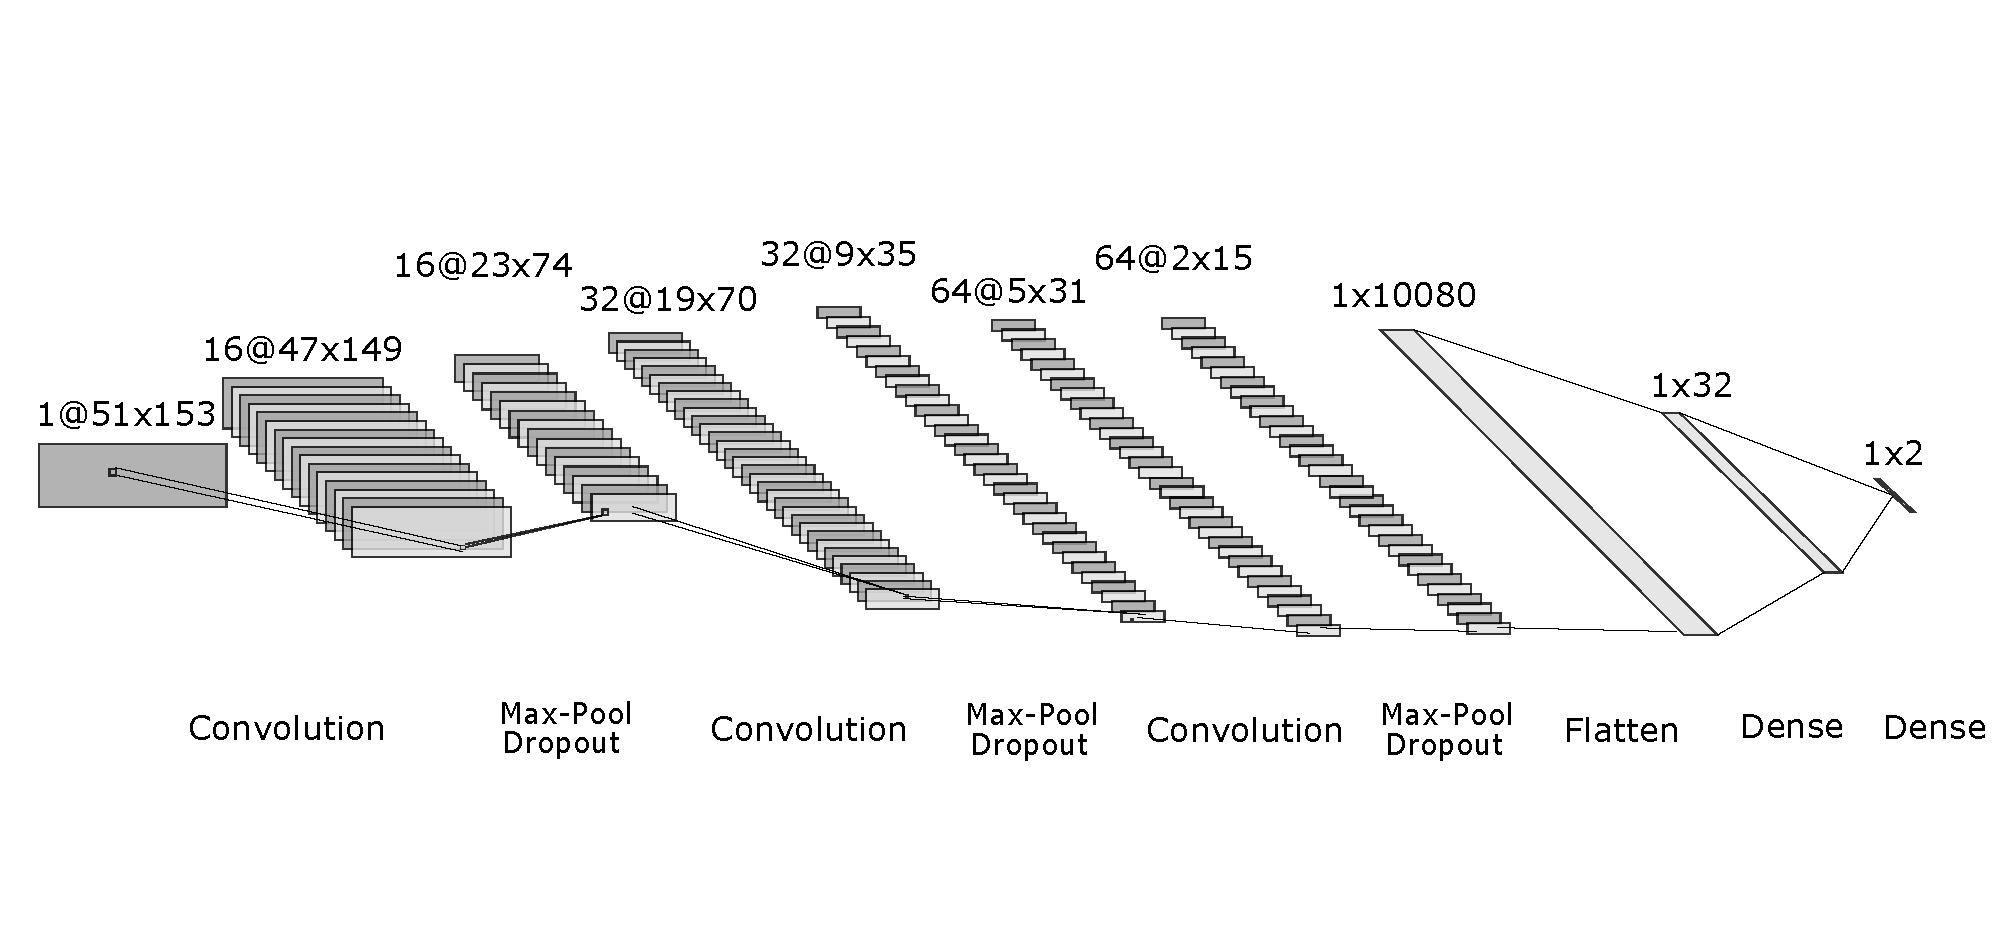
\includegraphics[width=0.45\linewidth]{
    figures/aaa_big.pdf}
    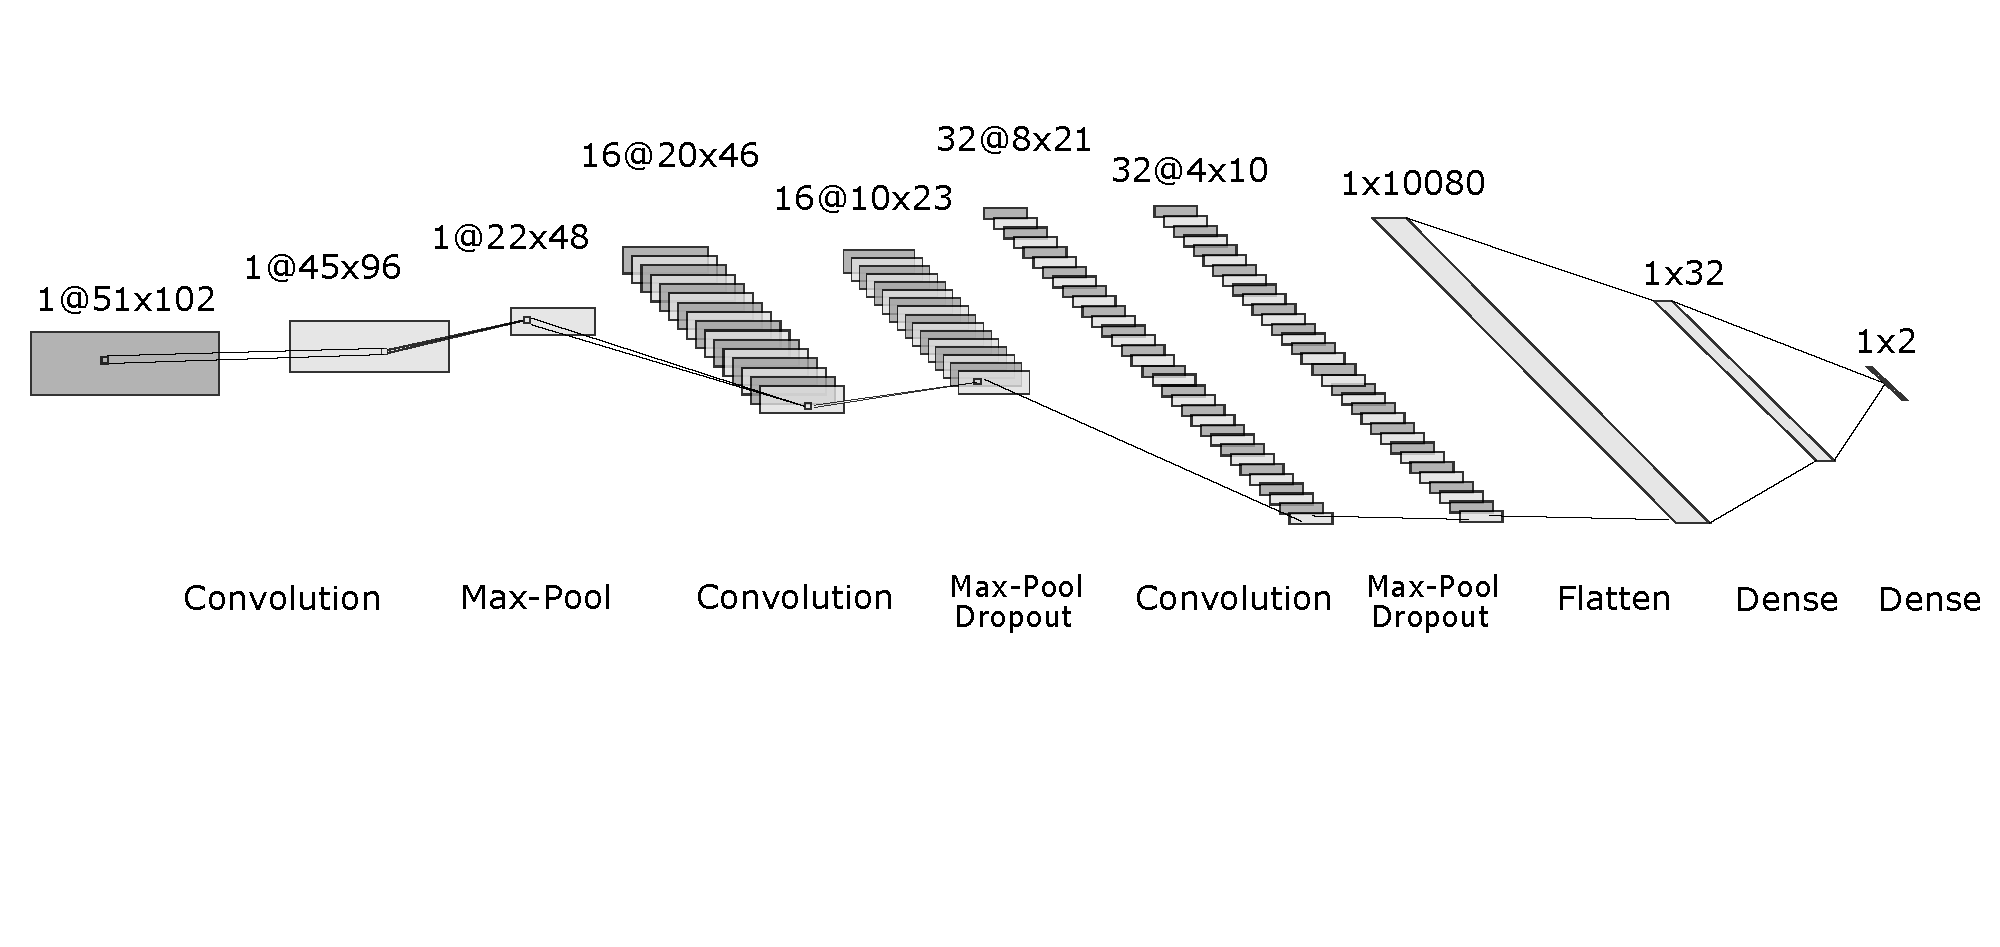
\includegraphics[width=0.45\linewidth]{figures/ccc_bug.pdf}
   \caption{Architecture of the Neural Networks used in this project to classify ``real'' and ``bogus'' transients. {\it Left}: the \diabased\ model that uses image triplets as input (\diff, \temp, \search). The input layer is $51 \times 153$ (see left \autoref{fig:examples_hstack_normalization}); a convolution layer $(5\times 5)$ learns $16$ filters; max pooling $(2\times2)$ and dropout; convolution $(5\times 5)$ learns $32$ filters;  maximum pooling $(2\times2)$ and dropout; convolution $(5\times 5)$ learns $64$ filters;  maximum pooling $(2\times2)$ and dropout; flatten layer, Dense $(32)$ and the output is a Dense $(2)$-class layer. {\it Right}: the \nodia\ model that uses the \temp\ and \search\ images only. The input layer is $51 \times 102$ (see right \autoref{fig:examples_hstack_normalization}); a convolution layer $(7\times 7)$ learns $1$ filter; maximum pooling $(2\times2)$; convolution $(3\times 3)$ learns $16$ filters;  maximum pooling $(2\times2)$ and dropout; convolution $(3\times 3)$ learns $32$ filters;  maximum pooling $(2\times2)$ and dropout; flatten layer, Dense $(32)$ and the output was a Dense $(2)$-class layer.The illustrations were made using NN-SVG tool by \citet{LeNail2019}.}
\label{fig:architecturesCNN}
\end{figure*}


One further decision has to be made in combining the three images in the DIA set to feed them to the CNN. We stacked the scaled \diff, \search\ and \temp\ horizontally. %  the three each image (already standardized and scaled) per ``ID'', following the order (\diff, \search, \temp), and using \textit{np.concatentate}; 
Thus the size of the data in input to our CNN is ($N_{tr}\times51\times153$), where $N_{tr}$ is the number of transients to be considered. Four examples of the data ``triplets'' in input to our \diabased\ CNN are in the left panel of \autoref{fig:examples_hstack_normalization}. Following this horizontal structure, we mimic closely the way that human scanned this type of data for classification, and we will take advantage of this scheme when examining the models' decisions in \autoref{subsec: saliency}, although stacking the images along a third depth axis has also been tested, with no differences in the model accuracy, \tatiana{with an accuracy also of 96\%.} \tatiana{See \hyperref[sec:appendix3channel]{Appendix B}.} %this acc is for CAVINESS, plots here are NERSC, acc is down by a ~1% using CAVINESS, NERSC is a lit less than 97%

But our goal is to test the performance of models that do not use the DIA. Thus for our \nodia\ models the training and testing data set were constructed in the same way as the previous triplets, but without the \diff\ image. Some examples are in the right panel of \autoref{fig:examples_hstack_normalization}.




% \onecolumngrid